%牛顿—莱布尼兹公式

\pentry{不定积分\upref{Int},定积分\upref{DefInt}}

牛顿--莱布尼兹公式描述了定积分和不定积分的关系.我们已知不定积分是求导的逆运算,而定积分是函数曲线下方的面积,二者乍看起来没什么联系,但牛顿-莱布尼兹公式却揭示了了二者之间的重要关系.

若 $F(x)$ 是 $f(x)$ 的一个原函数\upref{Int},则
\begin{equation}\label{NLeib_eq1}
\int_a^b f(x) \dd{x}  = F(b) - F(a)
\end{equation}

\subsection{推导}
\begin{figure}[ht]
\centering
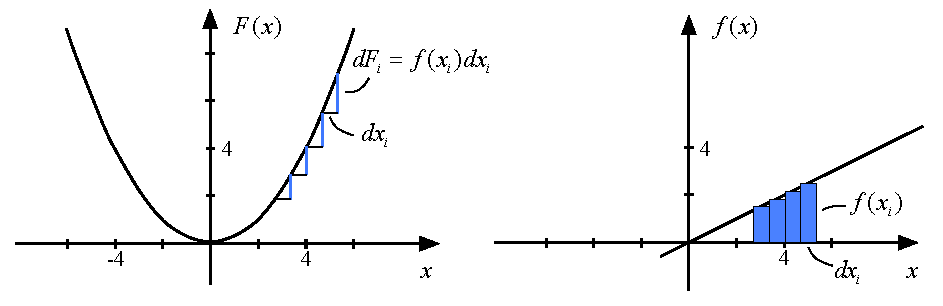
\includegraphics[width=13cm]{./figures/NLeib.pdf}
\caption{右图中 $f(x)$ 的原函数为左图中的 $F(x)$, 当步长趋近0时,右图中的长方形面积趋近于左图中小竖线的长度.}\label{NLeib_fig1}
\end{figure}

如\autoref{NLeib_fig1}, 根据定积分\upref{DefInt} 的定义,有\footnote{这里假设极限存在.}
\begin{equation}
\int_a^b f(x) \dd{x}= \lim_{\Delta x_i\to 0}\sum_i f(x_i)\Delta x_i
\end{equation}
其中 $f(x_i)\Delta x_i$ 可看成是右图中第 $i$ 个小矩形的面积,求和是对从 $a$ 到 $b$ 的所有小矩形求和.现在不妨把 $x_i$ 设为第 $i$ 个小矩形左端的 $x$ 坐标. 考虑到求导是不定积分的逆运算,有 $f(x_i)=F'(x_i)$, 所以小矩形的面积变为
\begin{equation}
f(x_i)\Delta x_i = F'(x_i)\Delta x_i \simeq \Delta F_i = F(x_{i+1})-F(x_i)
\end{equation}
最后一步使用了微分近似. %链接未完成
该式可以理解成,右图中的小矩形面积约等于左图中的小竖线长度,即原函数 $F(x)$ 在 $x_i$ 到 $x_{i+1}$ 间的增量.当取极限 $\Delta x_i \to 0$ 时,上式取等号.代回\autoref{NLeib_eq1}, 有
\begin{equation}
\int_a^b f(x) \dd{x}= \lim_{\Delta x_i\to 0}\sum_i [F(x_{i+1})-F(x_i)] = F(b)-F(a)
\end{equation}
该式可理解为,如果把左图中每一段 $\Delta x_i$ 所对应的微小增量 $\Delta F_i$ 都加起来,再取极限 $\Delta x_i \to 0$, 就是 $F(x)$ 从 $a$ 到 $b$ 的总增量.
% 未完成: 介绍 |_a^b 的意思! 也记为 [ ]_a^b


% 下面应该举一个 sin(x)^2 从 0 到 pi 的积分,既可以从原函数得出,也可以从几何对称性进行验证.
\begin{exam}{计算定积分}
\begin{equation}
\int_{m\pi}^{n\pi} \sin^2(\frac{n\pi}{l} x) \dd{x}
\end{equation}
先计算对应的不定积分.由积分表得 $\sin(x)$ 的原函数为 $-\cos(x)$, 由第一类换元法中式() % 未完成
得 $\sin(ax)$ 原函数为 $-\cos(ax)/a$. 所以
\begin{equation}
\int\sin^2(\frac{n\pi}{l} x) \dd{x} = \frac{1}{2}(x - \sin x\cos x) + C
\end{equation}
% 链接未完成
原函数
值得指出,另一种更简单的方法是,由于被积函数的对称性,可将一个周期内高为 1 的长方形(面积为 $\pi$ )划分成等面积的两部分,曲线下方的面积 $\pi /2$ 就是积分结果.% 图未完成
\end{exam}
